\section{Osrank}
\label{s:osrank}

% TODO(james):
%  - Net of deps, etc.
%  - Page surfer, deps was too directed, explain why we added contribution edges?

\def\Graph{\mathsf{Graph}}
\def\proj{\mathsf{proj}}
\def\user{\mathsf{user}}
\def\dep{\mathsf{dep}}
\def\own{\mathsf{own}}
\def\coown{\mathsf{own}^\circ}
\def\contrib{\mathsf{contrib}}
\def\cocontrib{\mathsf{contrib}^\circ}

Since one of the fundamental mechanisms of \oscoin{} is to distribute a portion
of newly minted \oscoin{} to high-value projects on the network, the protocol
needs to reach consensus on which projects are ``high value''. To choose which
projects receive \oscoin{}, and in which proportions, the network uses
\osrank{}, which is a modification of the well-know \pagerank{}
algorithm~\cite{pagerank} applied to the graph of relationships between
projects and contributions on the network, and in particular
\emph{dependencies} between projects. The output of the algorithm is a score
$\omega(P)$ associated to each project $P$.

\subsection{Rationale}

While it may be clear that value is being produced by a system as a whole, it is
often unclear how much value particular subsystems are
contributing. Furthermore, subsystems have inherently differing capacities to
transform value into revenue: subsystems at the boundaries with other domains
are at an advantage, even though they may (transitively) derive much of their
value from other subsystems. This disbalance in value flows in and out of
subsystems is detrimental to the system as a whole.

Thankfully, human activity does not happen in a void\footnote{Space
  exploration will be addressed in a subsequent paper.}: be it
knowledge work, content/media creation, financial activity, etc.,
entities interact with one another in meaningful ways that are highly
influenced by the relative value each entity has with respect to the
system as a whole. Crucially, during this activity, a trail of
\emph{artefacts} (hypermedia links, contracts, transactions,
dependencies etc.) is produced; concrete manifestations
of the relationships between the various entities.

% TODO: Re-order above two paragraphs?

The basic insight of \pagerank{} and similar metrics, is that by
stochastic simulation of meaningful activity traces of system agents,
producing trails of artefacts consistent with observations, one can
learn about the value flows between subsystems, and hence approximate
the underlying value distribution. In the case of \pagerank{} one
simulates a human searching for high-relevance data over the internet,
following a chain of links. A sophisticated algorithm would use as
many heuristics as possible for choosing the next link to follow (as a
real human would), \eg{} evaluating the relevance of the link-text. If
computational resources are scarce, the crudest algorithm simply picks
the next link at random, and this is what produces the classic
\pagerank{} formula which has seen so much success at ranking web
pages.

\subsection{Ranking entities in \oscoin{}}

The artefacts related to OSS development which are captured on the \oscoin{}
ledger are:
\begin{itemize}
  \item Ownership of a project by a key,
  \item Dependencies between projects,
  \item Contributions of code from users to projects.
\end{itemize}

\begin{center}
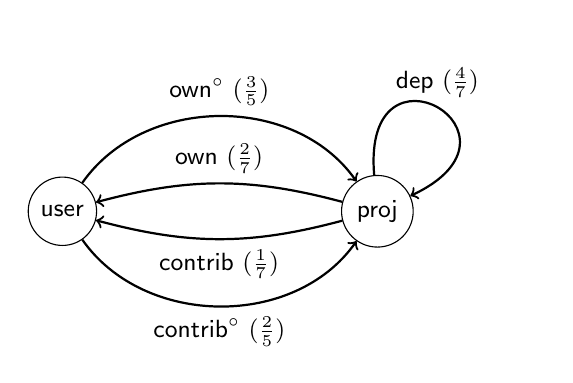
\begin{tikzpicture}[vertex/.style={draw,circle}, arr/.style={draw,thick,->}]
  \node[vertex] (p) at (2,0)  {\small $\proj$};
  \node[vertex] (u) at (-2,0) {\small $\user$};

  \draw[arr,looseness=9] (p) to[out=95,in=25] node[above] {\small $\dep \ (\frac{4}{7})$} (p);
  \draw[arr] (p) to[out=165,in=15] node[above]   {\small $\own \ (\frac{2}{7})$} (u);
  \draw[arr] (u) to[out=55,in=125] node[above]   {\small $\coown \ (\frac{3}{5})$} (p);
  \draw[arr] (p) to[out=195,in=-15] node[below]  {\small $\contrib \ (\frac{1}{7})$} (u);
  \draw[arr] (u) to[out=-55,in=-125] node[below] {\small $\cocontrib \ (\frac{2}{5})$} (p);
\end{tikzpicture}
\captionof{figure}{\small Entity relations in open source software development with example weights.\label{fig:G}}
\end{center}

% TODO: Can we avoid the term "user" here? Or mention that we aren't "ranking"
% users, intentionally.

We summarise these interactions with a weighted directed graph $G$
(Figure~\ref{fig:G}), the weights corresponding to the relative importance of
the edge, which can be set as parameters to the algorithm.

% TODO: include simulations description and results here.

The weights on all edges outgoing from a vertex sum to $1$.

Note that some of the edges are biderectional, but each direction gets
its own weight. For example both $\contrib$ and $\cocontrib$ pertain to
the same artefact: a contribution of code from a user to a
project. The edge $\contrib$ represents the statement \emph{the user
  is valuable to the project}. The edge $\cocontrib$ going in the
opposite direction represents the statement \emph{the project is
  valuable to the user}; the rationale for this less obvious flow is
that users are unlikely to invest time contributing to a project they
don't find useful.

% TODO: Make the above easier to grasp. Also maybe rephrase a little "is
% valueable to the project"

The \oscoin{} network proposes to record these artefacts as
transactions in a blockchain, so that one may unambiguously rebuild
and reach consensus on a finite directed graph $\netgraph$ over $G$
(\ie{} in the slice category $\Graph/G$). We'll refer to $\netgraph$
as the \emph{network graph}.

This in turn allows global value scores to be assigned to entities
according to a specific stochastic process simulating \emph{random
  walks}, that is, activity traces in $\netgraph$ with sampling
probabilities taken from $G$. For example: a contributor decides to
work on a high value project (probably at the border), contributes a
changeset, in so doing adds a dependency to another project, which imports a
bug from upstream. The contributor therefore switches to fixing said
bug in the dependency, etc. Much like a simulation of a human
searching for information by clicking through links, this simulated
contributor activity informs us on the value flows between subsystems
in OSS development.
% TODO: I think the above example mixes too many value flows.

This score, which we call \osrank{}, is used to weight the
distribution of newly minted tokens to high value entities, thus
compensating entities which bring value to the ecosystem.

\subsection{Definition}

To implement \osrank{}, we use the following Monte Carlo-based algorithm: for each
project on the network, $R$ random walks are performed which start at that
node. To decide which next vertex to visit during a random walk, first a type of
outgoing edge is decided by sampling outgoing edges according to the weights in
$G$. The next choice is specific to the edge:

\begin{itemize}
\item In the cases of $\dep$ and $\own$, all vertices are equiprobable.
\item In the cases of edges $x \xrightarrow[]{\coown} p$ and
  $x \xrightarrow[]{\cocontrib} p$ outgoing from a user $x$, a project $p$ is
  chosen with probability $\frac{p_x}{N_x}$, where $p_x$ is the number of
  contributions $x$ has contributed to $p$, and $N_x$ is the total number of
  contributions by $x$.
\item In the case of edges $p \xrightarrow[]{\contrib} x$, the users $x$ are
  chosen with probability $\frac{p_x}{N}$, where $N$ is the total number of
  contributions $p$ has received from all users.
\end{itemize}
% TODO: ^ Should it be "proportion of total contributions"?

At each step the walk might terminate with probability $1 - \epsilon$, (here
$\epsilon$ is the \emph{damping factor}, $0 < \epsilon < 1$). This produces a
set $W$ of walks. The \osrank{} for a project $x$ is then:
\[
  \omega(x) = \frac{W_x \epsilon}{n R}
\]
where $W_x$ is the number of visits of $x$, over all walks, that is:
\[
W_x = \sum_{w \in W} v(w,x)
\]
where $v(w,x)$ is the number of times path $w$ visits the vertex $x$.
% TODO: ^ Rephrase

\subsection{False ecosystems}

The main problem to avoid is compensating illegitimate ecosystems, that is,
project structures and relationships which have been setup in the
network graph for the sole purpose of exploiting the \osrank{} algorithm.

% TODO: Reference PageRank sybil attack papers
% TODO: Give example of "illegitimate" sub-graphs

For this we propose running \osrank{} in two distinct phases:
% TODO: We propose a modification of the page rank algorithm, based on TrustRank
\begin{itemize}
\item In the first phase, a seed set $\seedset$ is used as the [TODO] for the
  beginning of all walks. Specifically, a random walk always starts at
  a vertex in $\seedset$. Otherwise the process remains the same. The scores
  obtained are biased towards interactions with the seed set, but they
  are not used directly by the compensation mechanism. Instead a
  threashold $t$ is used to determine the legitimacy of entities: any
  entity falling below this threshold is not considered for the next
  phase. The output of this phase is a subgraph $\netgraph_t$ of the network
  graph.
  % TODO: Use of words: "entity" or "vertex"?
\item In the second phase, the algorithm is run on the subgraph
  $\netgraph_t$ as usual, with no seed set. The output of the second
  phase is the \osrank{}.
\end{itemize}

Care must be taken to ensure the seed set is large enough to touch most
legitimate projects on the network.  There are many ways to maintain such a
seed set. However, this will be discussed in future work.

\subsection{Implementation}

There are several options for making sure the computation of \osrank{}
will not be prohibitively expensive for network operators to run.
% TODO: Has "operators" been defined?

\begin{itemize}
\item \emph{Incremental Monte Carlo.} An incremental algorithm is used so that
  \osrank{} values may be updated as the network graph evolves. Instead of
  computing \osrank{} from scratch, we rely on the fact that only a small
  percentage of the nodes and edges of the network graph are added or removed
  from one calculation to the next (confirmed empirically on the datasets of
  major code-hosting platforms). Therefore most of the random walks that were
  performed in the previous calculation remain valid in the updated graph. For
  example if only a single dependency $p_1 \xrightarrow[]{\dep} p_2$ has been
  added since the last calculation, then a random walk that was generated on the
  old graph is only invalid in the updated graph if it passes through $p_1$, for
  it may have chosen to follow this new dependency to $p_2$.

  In practice the operators of the network cache the set of random
  walks from the previous calculation, and update this set by removing
  invalid walks and replacing them with new ones. Details on such an
  incremental algorithm used in the case of \pagerank{} can be found
  in \cite{incr pagerank}.

  Since all the computations must be deterministic, the walks are not
  truly random. Rather, they must use a built-in pseudo-random number
  generator to generate the random walks. The seed for generating
  random walks is fixed in the genesis block.

  % TODO: Add details on RNG

\item \emph{Long epoch.} In this scenario payouts according to
  \osrank{} are only made infrequently, say with a duration of $d$
  between \emph{payout} blocks (e.g.\ once every month). In this case
  abusers might modify network structures of several projects in
  anticipation of the payout block. To mitigate this, some edges are
  weighted by the amount of time they have existed in the last epoch. For
  example, if a dependency is added a day before the payout block,
  then it only has a weight proportional to $1/d$.
\end{itemize}

% TODO: Add closing statement/conclusion
